%%%%%%%%%%%%%%%%%%%%%%%%%%%%%%%%%%%%%%%%%
% Stylish Article
% LaTeX Template
% Version 2.2 (2020-10-22)
%
% This template has been downloaded from:
% http://www.LaTeXTemplates.com
%
% Original author:
% Mathias Legrand (legrand.mathias@gmail.com)
% With extensive modifications by:
% Vel (vel@latextemplates.com)
%
% License:
% CC BY-NC-SA 3.0 (http://creativecommons.org/licenses/by-nc-sa/3.0/)
%
%%%%%%%%%%%%%%%%%%%%%%%%%%%%%%%%%%%%%%%%%

%----------------------------------------------------------------------------------------
%	PACKAGES AND OTHER DOCUMENT CONFIGURATIONS
%----------------------------------------------------------------------------------------

\documentclass[fleqn,10pt]{SelfArx} % Document font size and equations flushed left

\usepackage[english]{babel} % Specify a different language here - english by default
\usepackage{pgfgantt}

\usepackage{lipsum} % Required to insert dummy text. To be removed otherwise

%----------------------------------------------------------------------------------------
%	COLUMNS
%----------------------------------------------------------------------------------------

\setlength{\columnsep}{0.55cm} % Distance between the two columns of text
\setlength{\fboxrule}{0.75pt} % Width of the border around the abstract

%----------------------------------------------------------------------------------------
%	COLORS
%----------------------------------------------------------------------------------------

\definecolor{color1}{RGB}{0,0,90} % Color of the article title and sections
\definecolor{color2}{RGB}{0,20,20} % Color of the boxes behind the abstract and headings

%----------------------------------------------------------------------------------------
%	HYPERLINKS
%----------------------------------------------------------------------------------------

\usepackage{hyperref} % Required for hyperlinks

\usepackage{makecell}
\hypersetup{
	hidelinks,
	colorlinks,
	breaklinks=true,
	urlcolor=color2,
	citecolor=color1,
	linkcolor=color1,
	bookmarksopen=false,
	pdftitle={Title},
	pdfauthor={Author},
}

%----------------------------------------------------------------------------------------
%	ARTICLE INFORMATION
%----------------------------------------------------------------------------------------

\JournalInfo{Laboratory of biological data mining} % Journal information
\Archive{Project proposal} % Additional notes (e.g. copyright, DOI, review/research article)

\PaperTitle{Identification and validation of a vitamin D related prognostic signature in colorectal cancer} % Article title

\Authors{Diego Barquero Morera\textsuperscript{1}, Giacomo Fantoni\textsuperscript{2}, Gaia Faggin\textsuperscript{3}, Leonardo Golinelli\textsuperscript{4}} % Authors
\affiliation{\textsuperscript{1}\textit{diego.barqueromorera@studenti.unitn.it}} % Author affiliation
\affiliation{\textsuperscript{2}\textit{giacomo.fantoni@studenti.unitn.it}} % Author affiliation
\affiliation{\textsuperscript{3}\textit{gaia.faggin@studenti.unitn.it}} % Author affiliation
\affiliation{\textsuperscript{4}\textit{leonardo.golinelli@studenti.unitn.it}} % Author affiliation

\Keywords{} % Keywords - if you don't want any simply remove all the text between the curly brackets
\newcommand{\keywordname}{Keywords} % Defines the keywords heading name

%----------------------------------------------------------------------------------------
%	ABSTRACT
%----------------------------------------------------------------------------------------

\Abstract{Colorectal cancer (CRC) is one of the most common malignant carcinomas worldwide with a poor prognosis, imposing an increasingly heavy burden on patients. Different studies have shown that vitamin D and vitamin D-related genes play a key role in CRC.
In this study we aimed to identify and validate vitamin D related prognostic signature in colorectal cancer.
In the first part of our work we will focus on the normalization and the preprocessing of our datasets: a colorectal cancer gene expression data datasets and a vitamin D level gene expression data datasets. Regarding the first dataset we will split the data in “stage I and II gene expression data” and “stage III and IV” gene expression data; while for the second dataset we will split the data in “low vitamin D level gene expression data” and “high vitamin D gene expression data”.
Then by the means of a statistical analysis will obtain a dataset of differential expressed genes in different stages of colorectal cancer and a dataset of vitamin D gene signature.
After that, we will intersect these two datasets in order to obtain our genes of interest. With this list of genes we will be able to perform a pathway enrichment analysis in order to extend our list of genes of interest. At this point, we will be able to compare the level of expression of genes of interest with patient data and fit a regression model for patient data prediction.
This regression analysis, once validated will allow us to obtain a list of genes significative for the stratification and prognosis of patients suffering from colorectal cancer.
}
%----------------------------------------------------------------------------------------

\begin{document}

\maketitle % Output the title and abstract box

\tableofcontents % Output the contents section

\thispagestyle{empty} % Removes page numbering from the first page

%----------------------------------------------------------------------------------------
%	ARTICLE CONTENTS
%----------------------------------------------------------------------------------------

\section*{Introduction} % The \section*{} command stops section numbering

\addcontentsline{toc}{section}{Introduction} % Adds this section to the table of contents

Colorectal cancer (CRC) is the third most common malignant tumor worldwide and is the second one in cancer-related deaths [1]. In spite of improvements in the management and treatments of patients with CRC in the last two decades, no satisfactory therapy exists when the surgery is not curative. The poor prognosis and the increasing incidence of CRC have provided strong motivation to construct a predictive model in CRC patients, which will benefit personalized treatment in clinical management [2].
There are lot of epidemiological and preclinical studies that indicate a beneficial effect of vitamin D on CRC incidence and mortality [3] [4].
Vitamin D is a fat-soluble vitamin and many genes are related to its metabolism and action [5]. It can be obtained from diet or the endogenous synthesis in the epidermis under sunlight exposure [6]. It has been demonstrated that vitamin D benefits clinical outcome and improves the long-term survival of CRC patients [7]. Moreover, circulating vitamin D may be a CRC biomarker and is deficiency is related to the high incidence of CRC [8].
A better survival outcome in CRC is associated with higher prediagnostic or postdiagnostic serum 25-hydroxyvitamin D concentrations [9]. The most active vitamin D metabolite (1$\alpha$,25-dihydroxyvitamin D3) inhibits the proliferation and promotes the differentiation of cultured colon carcinoma cells by mechanisms that include cell cycle arrest at G0/G1 phase, blockade of the Wnt/$\beta$-catenin pathway and induction of E-cadherin and other epithelial proteins [3] [10] [11].
Lots of genes are related to vitamin D metabolism and action, play an essential role in tumors. For example, CYP24A1 an important vitamin D-related gene, is up-regulated in CRC patient and nominated as a promising biomarker [12]. Vitamin D and its related genes are correlated with the homeostasis of the intestinal epithelium, regulate immune cells [13]

%------------------------------------------------

\section{Biological question}
The objective of this project is to try to find a way to make prognosis and stratify patients suffering from colorectal cancer by means of their transcriptomic profiles.
In particular we are focusing on the gene signature of vitamin D as a prognostic marker.
To do so we are leveraging the always increasing gene expression analysis data publicly available.
The data will be used to build and validate a statistical model that will be able to stratify patients according to their survival ability.
Moreover we are hoping to identify in this process some colorectal cancer survival markers related with vitamin D effects and pathways involved.


\section{Data}
Where we are looking for data, what data we have chosen and why, how it is going to be splitted.
Information about each dataset as in table \ref{tab:datasets}

\begin{table*}[ht]
	\centering
	\begin{tabular}{cccc}
		\hline
		Dataset name & Sample description & Number of samples & Usage \\
		\hline
		E-MTAB-6698	& healthy and tumor colorectal samples	&1566	&CRC DEGs\\
		GSE157982	&baseline and vit. D-treated CRC rectal samples	&98&	Vit. D signature\\
		GSE38832	&tumor colorectal samples	&122&	training and validation\\
		TCGA-COAD	&tumor colorectal samples	&438&	training and validation		\\
		GSE14333	&tumor colorectal samples	&290&	training and validation\\
		GSE17536	&tumor colorectal samples	&177&	training and validation	\\
		GSE31595	&tumor colorectal samples	&37	&training and validation	\\
		GSE33113	&tumor colorectal samples	&96	&training and validation	\\
		GSE38832	&tumor colorectal samples	&122&	training and validation	\\
		GSE39084	&tumor colorectal samples	&70	&training and validation	\\
		GSE39582	&tumor colorectal samples	&585&	training and validation	\\
		GSE103479	&tumor colorectal samples	&156&	training and validation	\\
		GSE17537	&tumor colorectal samples	&55	&training and validation	\\
		\hline
	\end{tabular}
	\caption{Datasets used}
	\label{tab:datasets}
\end{table*}

\section{Pipeline}
The project pipeline is described in figure \ref{fig:pipeline}.
\begin{figure}[ht]\centering % Using \begin{figure*} makes the figure take up the entire width of the page
	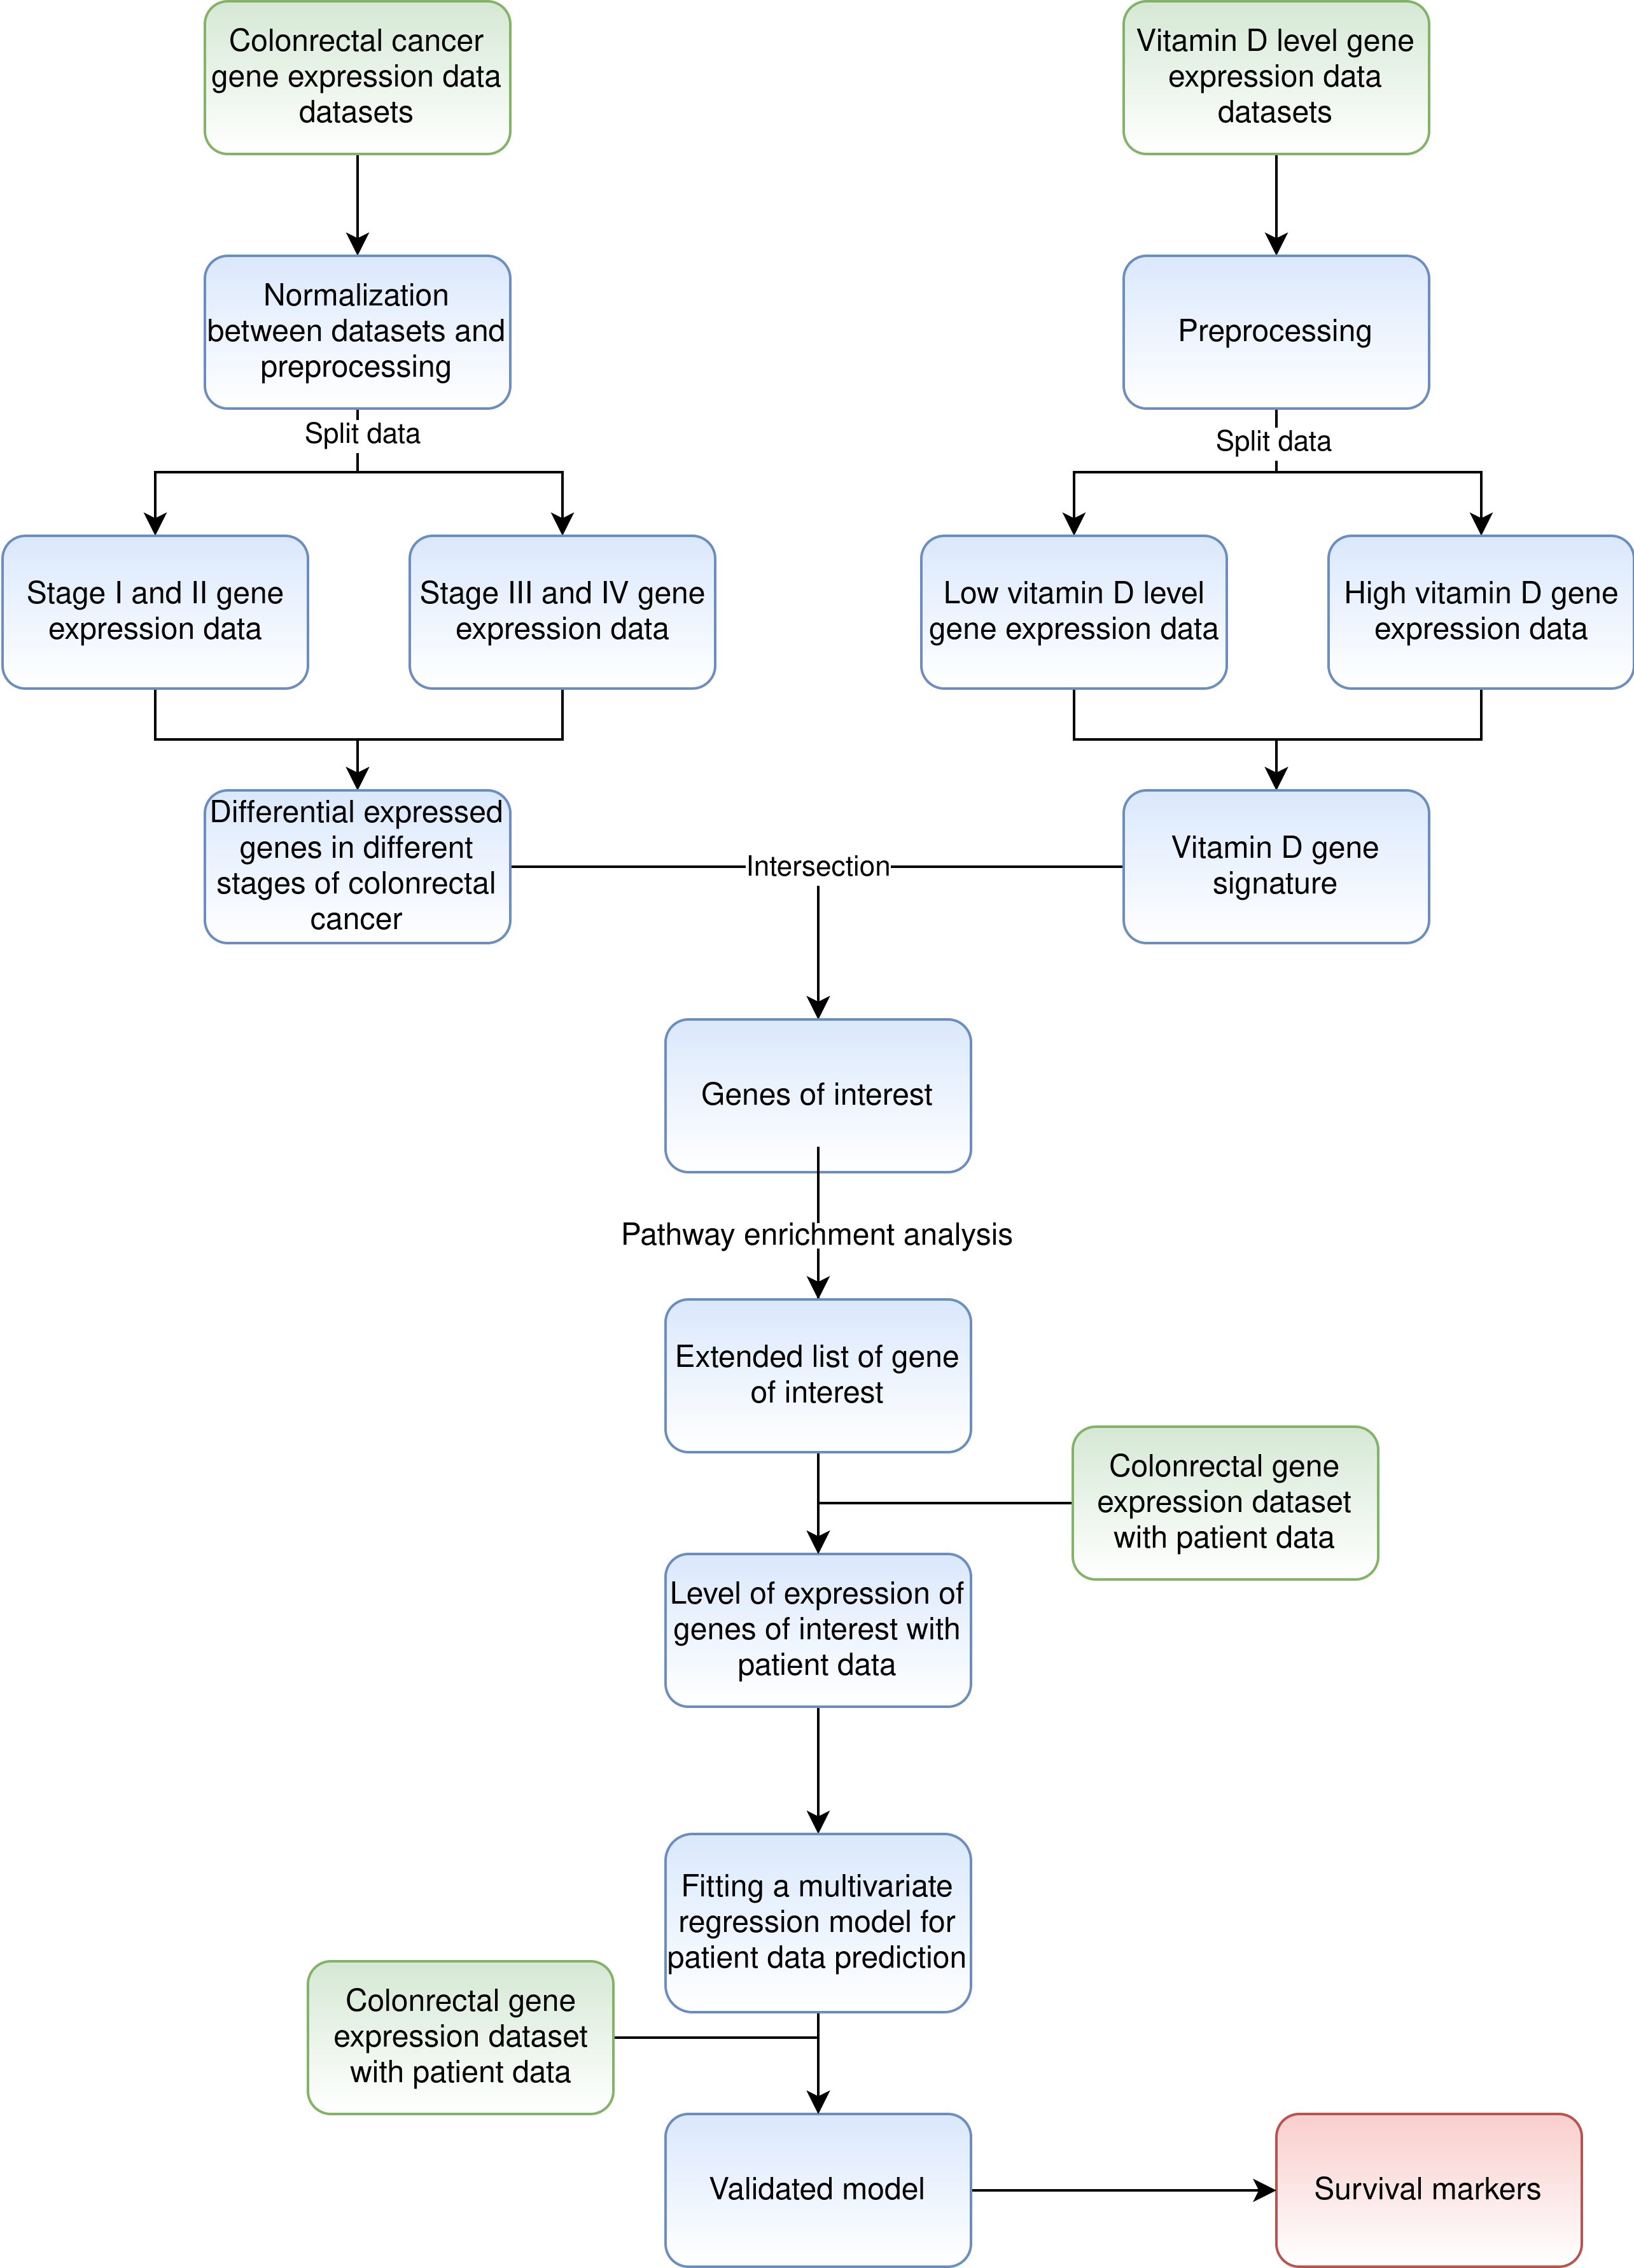
\includegraphics[width=\linewidth]{pipeline}
	\caption{Project pipeline}
	\label{fig:pipeline}
\end{figure}

	\subsection{Data preprocessing}

		\subsubsection{Normalization}
		Normalization is done to eliminate the batch effect because we are working with different datasets.
		We will try different algorithms and evaluate them to discover the better one.

		\subsubsection{Data filtering}
		Filter out samples without survival data or withouc comparable data distribution after normalization.

		\subsubsection{Evaluation of pre-processed data}
		The evaluation can be done using PCA, linear regression or hierarchical cluster analysis.

	\subsection{Obtaining the list of gene of interest}

		\subsubsection{Differential expressed genes between different stages of CRC}
		Split data in stage I and II gene expression data and in stage III and IV gene expression data, in order to obtain differential expressed genes in different stages of colorectal cancer.


		\subsubsection{Vitamin D gene signature in CRC}
		Split data in low vitamin D level gene expression data and in high vitamin D level gene expression data, in order to obtain vitamin D gene signature.


		\subsubsection{Intersection and enrichment}
		Intersection of the obtained datasets in order to obtain a subset of genes of interest. Pathway enrichment analysis for the identification of the classes of genes over-represented in our subset of genes.

	\subsection{Fitting to a regression model}
	Fitting a single variable or multivariate regression model for patient data in order to asses for each gene of interest its correlation with the stratification of the patient.

	\subsection{Obtaining of the survival markers}
	Retrieving from the fitted model those gene that presents a significative impact on patient stratification.

\section{Expected results}
A list of gene usable as survival marker in CRC.
According to (cite studies) possible candidates are:

\begin{table}[ht]
	\centering
	\begin{tabular}{cc}
		\hline
		Gene & Function\\
		\hline
		CYP24A1& temp\\
		TGFB1& temp\\
		IGFBP2& temp\\
		CYP24A1& temp\\
		CH25H& temp\\
		IGFLR1& temp\\
		DCBLD2& temp\\
		PTPN14& temp\\
		SLC10A2& temp\\
		FGF2& temp\\
		\hline
	\end{tabular}
	\label{tab:suvmark}
	\caption{Possible survival marker as found in literature}
\end{table}
\section{Project management}
The project will be developed in a dynamic and teamwork driven manner.
This is done in order to be able to leverage the particular skills and knowledge of each member.
Each task will be divided into the members in subtasks tailored according to his or hers background.
There will be frequent meetings with at least bi-daily cadence to asses progress and resolve problems.
Times estimates for each part are outlined in the chart \ref{chart:gantt}

\begin{figure}[ht]
	\label{chart:gantt}

	\begin{ganttchart}[hgrid,
		vgrid,
		title label font = \tiny,
		inline,
		time slot format=isodate,
		x unit=2mm,
		canvas/.style= { fill = green!25, draw =green!50, thick},
		bar/.append style={fill=red!50},
		title/.style={fill=yellow!50}
		]{2021-11-08}{2021-12-12}
		\gantttitlecalendar{month, day, week=1, weekday} \\
	\ganttbar{\makecell{Dataset \\normalization}}{2021-11-08}{2021-11-11}\\
	\ganttbar{\makecell{Normalization\\Evaluation}}{2021-11-12}{2021-11-18}\\
	\ganttbar{\makecell{Obtaining\\ DEGs}}{2021-11-19}{2021-11-22}\\
	\ganttbar{\makecell{Obtaining \\Vitamin D \\gene signature}}{2021-11-19}{2021-11-22}\\
	\ganttbar{\makecell{Pathway \\analysis}}{2021-11-22}{2021-11-28}\\
	\ganttbar{\makecell{Model selection \\ and fitting}}{2021-11-29}{2021-12-05}\\
	\ganttbar{\makecell{Model \\validation}}{2021-12-06}{2021-12-10}\\
	\ganttbar{\makecell{Survival\\ markers\\ analysis}}{2021-12-11}{2021-12-12}\\
	\ganttbar{\makecell{Report\\writing}}{2021-11-11}{2021-12-12}
\end{ganttchart}
\end{figure}
%------------------------------------------------


\phantomsection
\section*{Acknowledgments} % The \section*{} command stops section numbering

\addcontentsline{toc}{section}{Acknowledgments} % Adds this section to the table of contents


%----------------------------------------------------------------------------------------
%	REFERENCE LIST
%----------------------------------------------------------------------------------------

\phantomsection
\bibliographystyle{unsrt}
\bibliography{sample.bib}

%----------------------------------------------------------------------------------------

\end{document}
